\section{Supplementary Figures}

\begin{figure}[h]
\begin{center}
    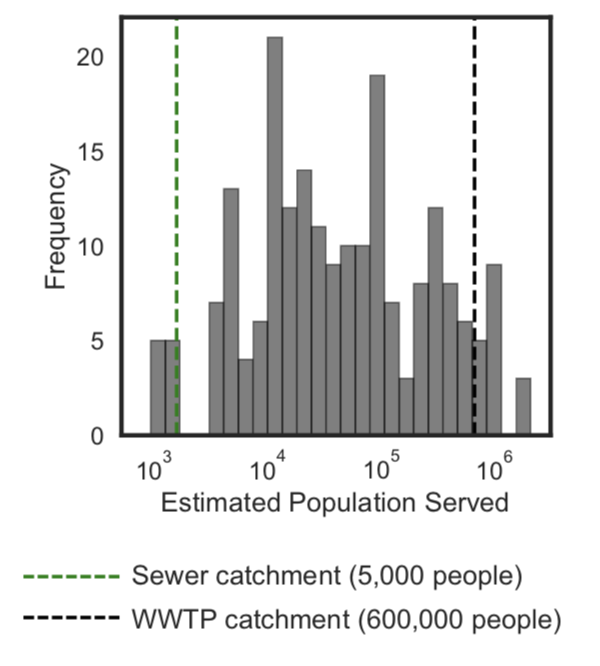
\includegraphics{s1_population_sizes_newton.png}
    \caption{Distribution of catchment sizes in Newton et al, 2015. Green dashed line indicates catchment size of upstream residential manhole and black dashed line indicates estimated catchment size of downstream site sampled in this study.}\label{24hr:figS1}
\end{center}
\end{figure}

\begin{figure}[h]
\begin{center}
    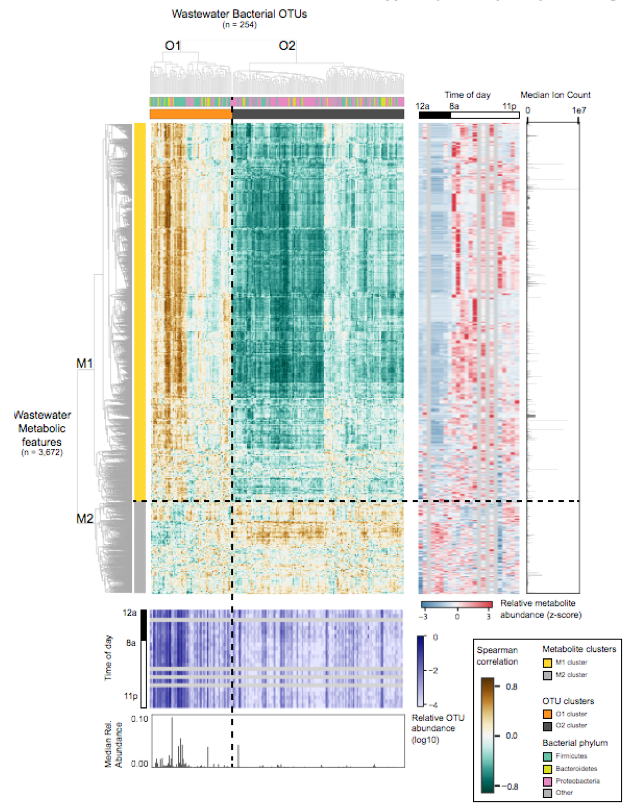
\includegraphics{s2_correlation_heatmaps.png}
    \caption{Co-clustering metabolomics and microbiome data identifies human-associated and environmental clusters. (Middle panel) Spearman correlation between metabolites and OTUs. (Right panel) Z-scored metabolite abundances over 24-hour sampling. Metabolites are in rows, time points are columns. Right-most panel shows daily median ion count of each metabolite feature. (Bottom panel) Heatmap of log10(relative abundance) for each OTU. OTUs are in columns, time points are rows. Bottom-most panel shows daily median relative abundance of each OTU.}\label{24hr:figS2}
\end{center}
\end{figure}

\begin{figure}[h]
\begin{center}
    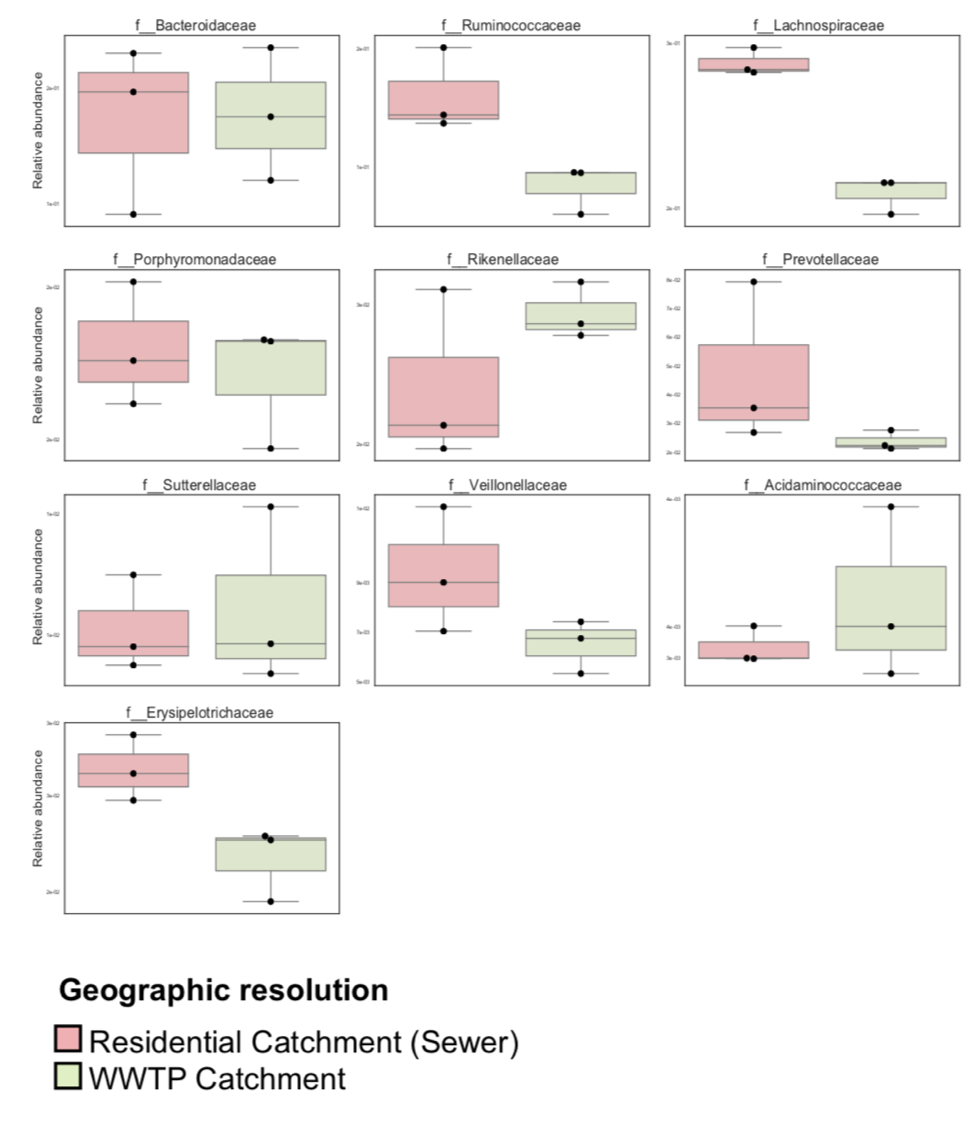
\includegraphics{s3_upstream_downstream_bacteria.png}
    \caption{Abundance of human-associated bacterial families in upstream vs. downstream sample.}\label{24hr:figS3}
\end{center}
\end{figure}

\begin{figure}[h]
\begin{center}
    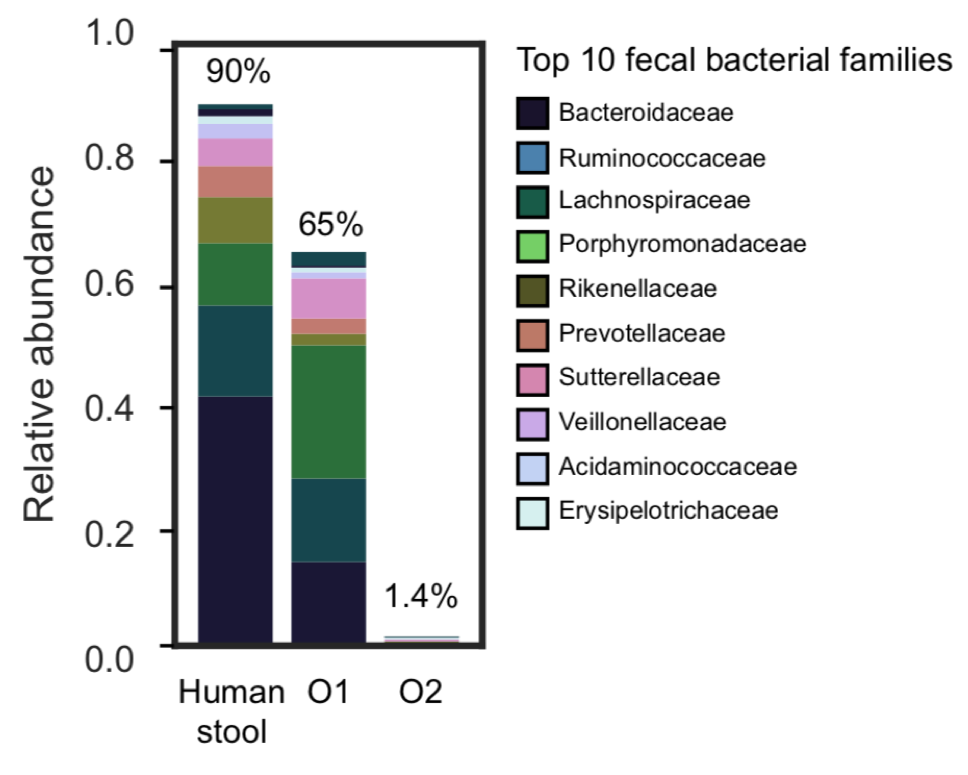
\includegraphics{s4_o1_o2_upstream_downstream.png}
    \caption{Abundance of human-associated bacterial families in OTU clusters O1 and O2.}\label{24hr:figS4}
\end{center}
\end{figure}
